\chapter{Theory}


\section{Moon Characteristics} % JP, Yannis

\iffalse
* Rock core, water, ice

    * Why do we think so?
    
    * Geysers?
\fi 

\subsection{Radiation Environment} % Maja, "landing site guys", "orbiter guys"

%* Both for the orbiter and the lander

\subsection{Tidal Wave} % Lukas, KSL

\section{Ice characteristics} % Lukas, KSL, Rasmus


\subsection{Structural Profile}
The first space probe flybys took place in the early 1970s, and Europa quickly became one of the main focuses in the search for past or present extraterrestrial life-harbouring environments, within reachable distances. Already in the 1960's were it discovered from earth-based observations, that the surface of Europa was covered in solid ice, not much unlike other satellites located that deep in the cold reaches of our solar-system. However, data recovered from satellite flybys supplied us with new information about the geology and composition of the moon's surface, having since helped us understanding the of Jupiter's, arguably, most interesting moons with respect to life-supporting environments.\\
\\
The Voayger mission from the late 1970's sent back coarse imagery of Europa with resolution in the ranges of kilometres per pixel, carrying valuable information about the surface of the Jovian satellite\cite{VoyagImg}. More specifically, the images showed a surface resembling that of a ball of string, discarding theories of Europa having a smooth surface, with it in stead being full of bands and ridges.\\%See requested article from DTU Findit
The Galileo spacecraft was launched in 1989 and entered orbit around Jupiter in 1995. It started transmitting data back to earth, from its extensive remote-sensing instrument suite
\iffalse 
(seen on fig. \ref{fig:GalInst1} and \ref{fig:GalInst2})
\fi
 with resolution surpassing Voayger's images almost three orders of magnitude. 
\iffalse
\begin{figure}[htbp]
	\centering
	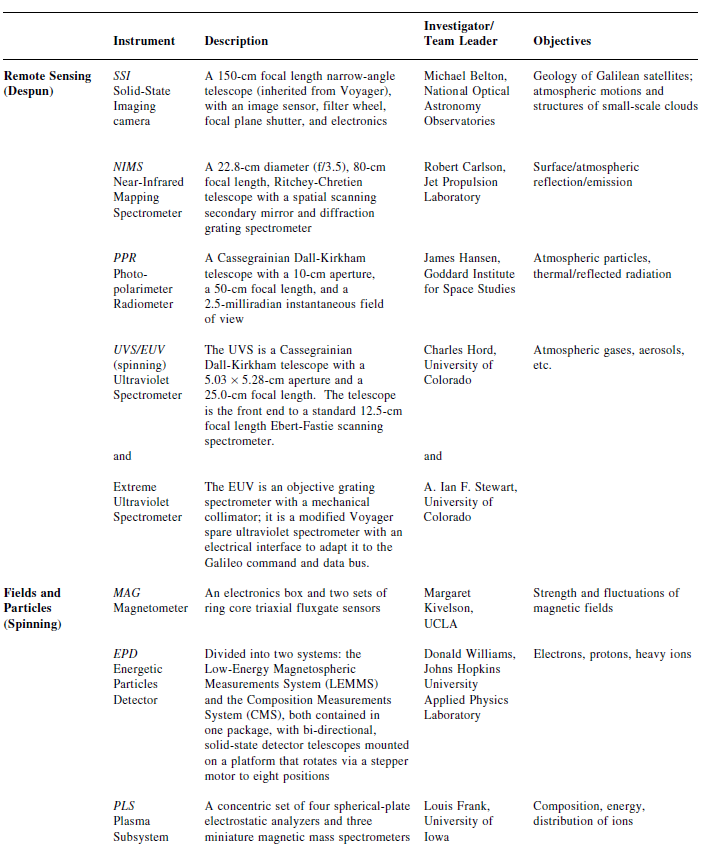
\includegraphics[width=\textwidth]{figures/Rasmus/GalileoInstrument1}
	\caption{Instrument suite of the 1989 Galileo mission.\cite{SciStrat} (\textit{Continued in fig. \ref{fig:GalInst2}}). \label{fig:GalInst1}}
\end{figure}
\begin{figure}[htbp]
	\centering
	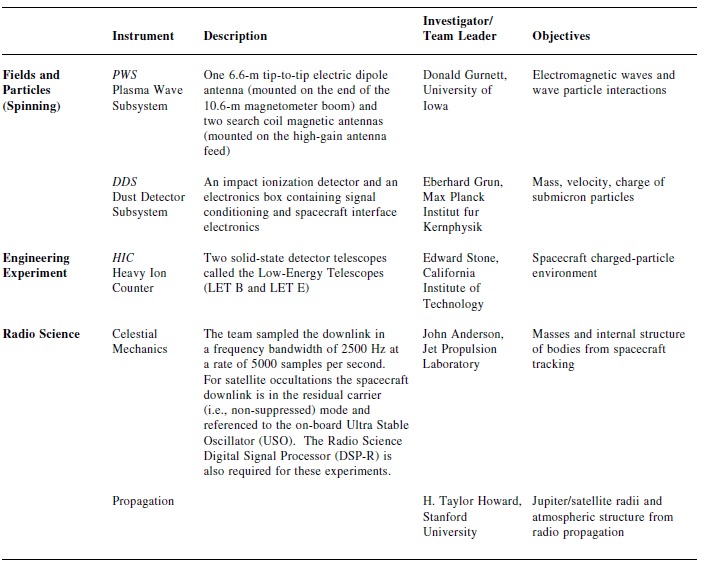
\includegraphics[width=\textwidth]{figures/Rasmus/GalileoInstrument2}
	\caption{Instrument suite of the 1989 Galileo mission.(Continued from fig. \ref{fig:GalInst1}) \cite{SciStrat} .\label{fig:GalInst2}}
\end{figure}
\fi
\\
The high-resolution measurements showed what seemed to be blocks of ice filled with ridges and/or early cracks, that had been lifted and rotated at some point in time. These disruptions indicates that there might be a liquid or softer slushy layer underneath the solid ice surface that through movement had broken and relocated the ice-crust. These cracks are illustrated on fig. \ref{fig:SurfCrack}, which is one picture of a series from the 1989 Galileo satellite\cite{HidOcean}. In any case, it indicates that there is some kind of structural activity in the outermost layer of the moon.\\
\\

\begin{figure}[htbp]
	\centering
	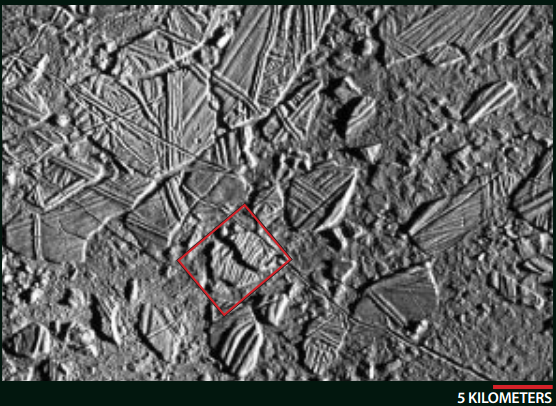
\includegraphics[width=\textwidth]{figures/Rasmus/SurfCrack}
	\caption{Image of Europa's surface taken by the Galileo satellite, showing ridges and disruptions in the surface. \label{fig:SurfCrack}\cite{HidOcean}}
\end{figure}

% Surface Composition
As explained in the study made by the Space Studies Board's Committee on Planetary and Lunar Exploration (COMPLEX), the data from Galileo’s Near-Infrared Mapping Spectrometer (NIMS) show that the water-ice absorption of Europa doesn't match with the expected outcome of pure-water ice, even for areas where the level of frozen sulfur oxide is thought to be lowest (The source of this $SO_2$ is presumably volcanic eruption on Io.). There has been some theories on the cause of this, including the presence of salts and other minerals in the ice but recent studies show that bubbles and fractions could result in the same discrepancies and band shifts in the measurements. However, it is still believed that some of the darker spots seen on the moon are observed because of salts and minerals like hexahedrite, epsomite, and natron\cite{SciStrat}. % INDSÆT The identity of that contaminant so far eludes scientists, but sulfur or iron compounds are suspected from Hidden Ocean P. 8
\\
\\
The actual thickness of the theorized ice-crust, and even the complete structural model of the moon, is still subject to many discussions. It was previously (prior to the Galileo mission) believed that the moon could be consisting of a hydrated silicate core coated in a thin layer of water-ice. However, with the measurements of Europa's gravitational field done by the Galileo satellite has this theory since been largely debunked. The current popular belief is that the cores is either a solid or fluid metallic core surrounded by a layer of water and ice of more than 100km due to the estimated density of the Jovian body. \\
The global ratio between liquid and solid water-ice is still unknown since it must be based on assumptions about the internal structure of the ice, which in themselves are extremely uncertain. The estimates we do have are even based on local imagery, since making them on a global basis requires dedicated orbiter mission, like the planned CLIPPER mission.\\%INDSÆT REFERENCE
In one study, the impact craters of Europa are analysed and compared with computer simulations to estimate regional crust thickness. The rationale is, that central peaks found in craters on the surface resemble material uplift caused by meteor impacts on extraterrestrial planets\cite{ThickImpact}, as seen on fig. \ref{fig:ImpactPic}. Therefore, it is assumed that the crust is thick enough to prevent complete surface penetration from meteor impact and as such they conclude that the ice at the impact sites must have been more than 	$\mathbf{3-4km}$ thick. Graphical representation of the simulation results can be seen on fig. \ref{fig:ImpactSim}. Another study that also investigated the impact craters, and taken from their introduction: "Stereo topographic profiles suggest that the plateau [a plateau SW of Cilix impact crater] is
flexurally supported, with an effective elastic thickness $t_e$ of
$~6km$. For a conductive temperature profile this $t_e$ value
implies a solid ice shell thickness of $\mathbf{~15km}$; if the shell is
convecting, this estimate is a lower bound. Combined with
independent estimates, we infer a probable shell thickness
of $\mathbf{25 km}$. The shell thickness is likely to be uniform over
the entire satellite."\cite{ThermElast}
\begin{figure}[htbp]
	\centering
	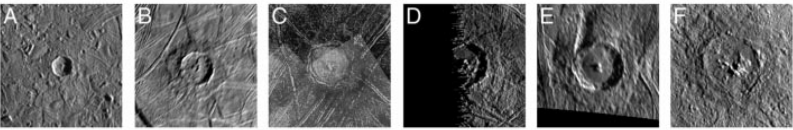
\includegraphics[width=\textwidth]{figures/Rasmus/Impacts}
	\caption{Galileo images of Europan central peak craters. (\textbf{A}) Brigid ($11^\circ$N, $80^\circ$W), $D=8.5km$. (\textbf{B}) Grainne ($60^\circ$S, $95^\circ$W), $D=13.5$km. (\textbf{C}) Cilix ($2.6^\circ$N, $182^\circ$W ), $D18.4$km. (\textbf{D}) Amergin ($14^\circ$S, $230^\circ$W), $D=18.6$km. (\textbf{E}) Maeve ($58^\circ$N, $75^\circ$W ), $D=20.4$km. (\textbf{F}) Pwyll ($25^\circ$S, $271^\circ$W), $D=23.7$ km. All images are at a resolution of 250 m/pixel and each is illuminated from the right except Cilix (\textbf{C}), which was observed at high sun
	\cite{ThickImpact}. D is crater diameter. \label{fig:ImpactPic}}
\end{figure}
\begin{figure}[h]
	\centering
	\includegraphics[width=1\textwidth]{figures/Rasmus/Impacts2}
	\caption{Model results for impacts of large (A through C) and small projectiles (D through F) into 9-km-thick ice (gray) over liquid water (A) and (D), 5-kmthick ice (gray) over liquid water (black) (B) and (E), and 3-kmthick conductive lid (light gray) over convecting ice (dark gray) (C) and (F). Solid, dotted, and dashed lines show the regions of complete vaporization, complete melting, and $50\%$ melting, respectively.
	\cite{ThickImpact}.\label{fig:ImpactSim}}
\end{figure}
\\
Thermal models has also been used to estimate the average ice shell thickness of Europa. One study is carried out with the assumption of a ice shell decoupled from a silicate core by a layer of liquid water \cite{ThermThick}, so its conclusion may not fit with modern theories. They estimate the shell to have a thickness of $\mathbf{13-25km}$, depending on which thermal rheology model is used (Maxwell and general flow rheology, with and without heat flow from the core). Another thermal model is based on the suggestios of Europa having a metallic core and a silicate mantle, covered by significant layer of liquid water and a thinner ice shell \cite{ThermThick2}. The study heavily relies on convection in the ice, and this complicates the study further. The heat flow through the ice is dependant on the shell thickness, and shell thickness is in turn dependant on the heat flow. This study concludes on the result that the average thickness of a completely frozen shell must be around $\mathbf{36km}$ based on the study's assumptions.
\\
\\ One study carried out by [J.M. Wahr, M.T. Zuber et al., 2006] analyses the tidal effects caused by the differentiating gravitational pull from Jupiter, as Europa travels in its elliptical orbit around the planet. The result of the study is a set of analytical equations estimating the global thickness based on the Love-number of Europa. However, in order to utilize these equations, accurate knowledge of the ice-composition is required, as well as precise estimates of the Love numbers. In the end they even conclude conclude that their results may not be sufficient since they only provide an accuracy of $\pm 5\mathrm{km}$.\\
\\
Apart from the thickness and elemental composition of the ice, internal structure in the shelf is also highly relevant to the planned penetrator mission. Assuming a completely homogeneous ice-shelf is a crude over-simplification and may be a mission-killer if alternatives aren't considered. 
\begin{figure}[h]
	\centering
	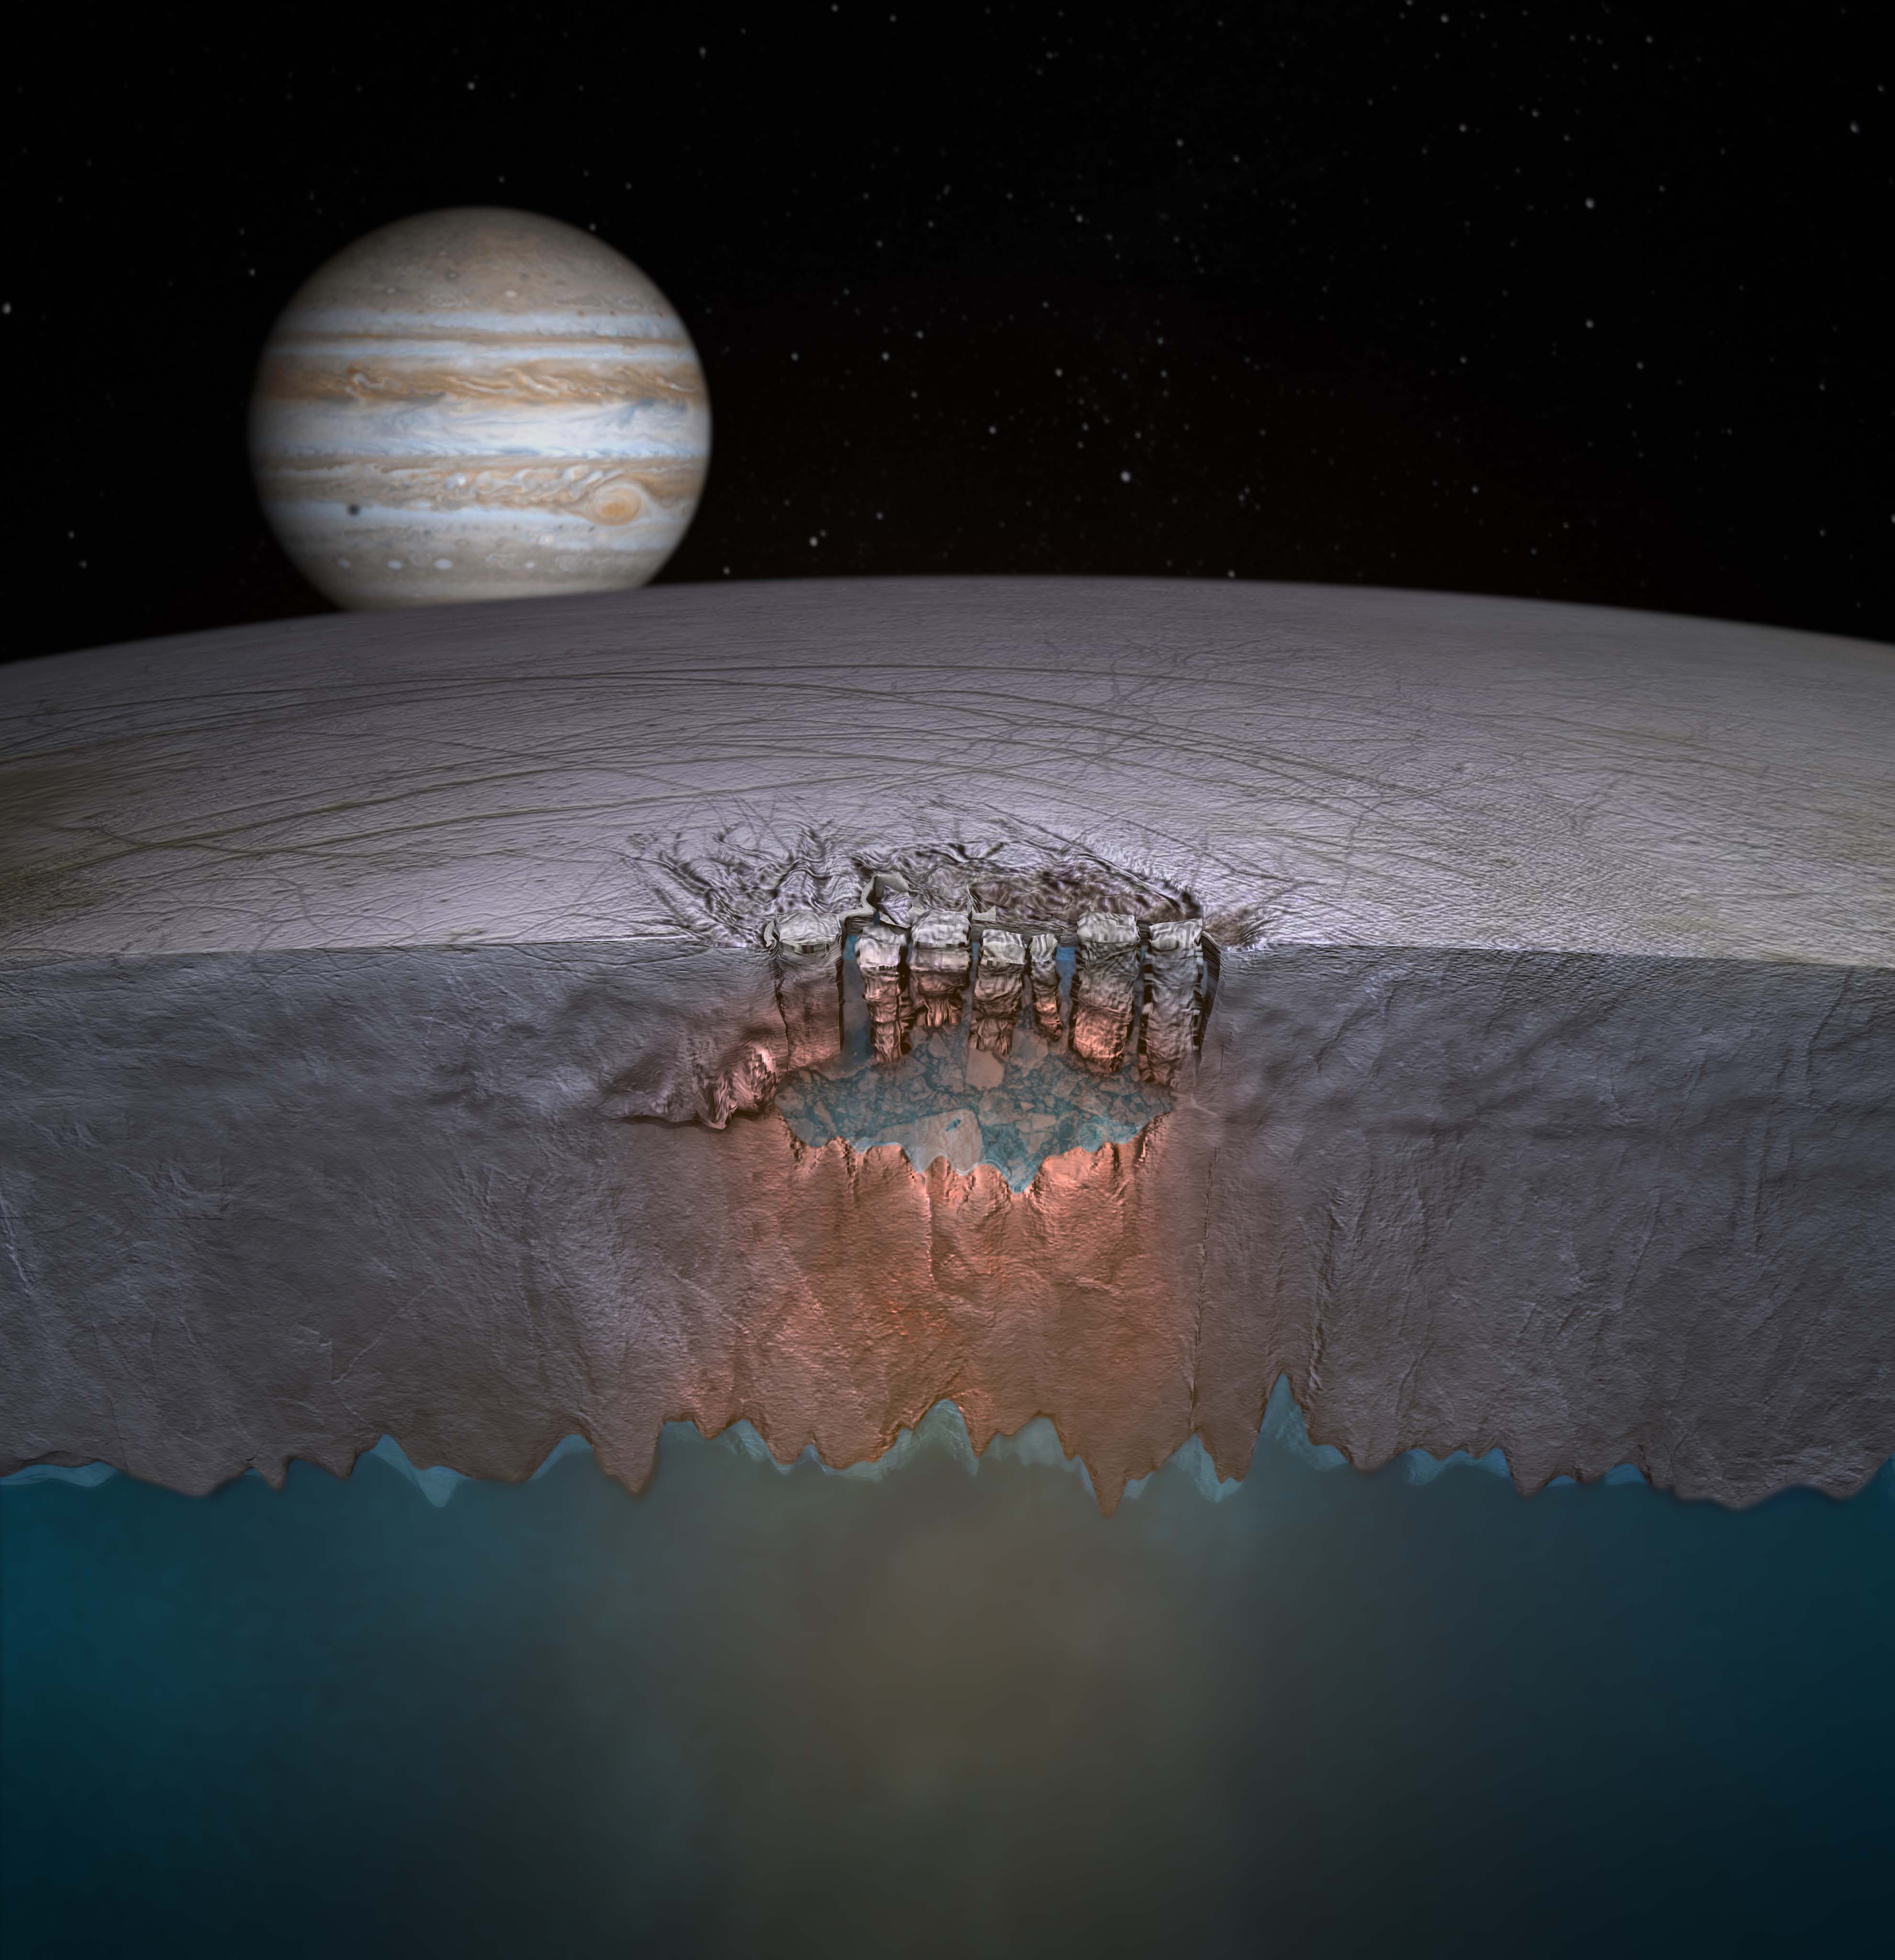
\includegraphics[width=0.5\textwidth]{figures/Rasmus/ArtLake}
	\caption{Artistic illustration of potential water lense, or lake, in the ice shell. \label{fig: ArtLake}}
\end{figure}
As such, apparent "Chaos Regions" has been observed on the surface of Europa and their causes has for a long time alluded scientists. However, recent studies suggests that these are formed due to water lenses in the shell, which can also be interpreted as lakes of liquid water \cite{IceLakes}. They way even be present within $3km$ of the surface, and it is estimated that there may be a water lense consisting of $20,000 - 60,000km^3$ of liquid water beneath the so-called Thera Macula chaos region. An artistic illustration of this phenomenon is shown on fig \ref{fig: ArtLake}.

\iffalse
* Ice thickness

* Composition of the ice? % Se: SWRI: "barr-showman-2009" (ask Kristian Lauszus)

* Lakes?
\fi

\subsection{Temperature Profile}

* "back of the envelope" calculations

\subsection{Pressure Profile}

* What is the outside pressure?

\subsection{Simulation Results}

\subsection{Simulation Validation}

* Should show that the "back of the envelope" calculations are right

\section{What Defines Life?} % Agge, Fruzsi

* Water, oil, fat, carbon, energy

* Proteins (amino acids) etc

* Nutritions, water, heat energy

* How can a life-form be able to convert thermal energy to other forms of energy

* Another energy source could be geysers on the solid core

    * A probe to the ocean bottom might show this
    
* Lakes inside the ice

* Iron-reduction

\subsection{Where do we expect to find life?}

* Top or bottom of the water?

* Petri Dish can be used for cultivation

* Steralization of the spacecraft: chemical, heat, radiation
